\documentclass[12pt, a4paper]{article}
\usepackage{fontspec}
\usepackage{amsfonts}
\usepackage{amsmath}
\usepackage{yfonts}
\usepackage{polyglossia}
\usepackage{graphicx}
\usepackage{xcolor}
%\usepackage{fourier}
\usepackage{hyperref}
\usepackage{ifthen}
\usepackage{marginnote}
\usepackage{pdfcomment}
\usepackage{accsupp}
\usepackage{ulem}
\usepackage[a4paper, margin=1in]{geometry}
\defaultfontfeatures{Ligatures=TeX}

\setdefaultlanguage{polish}
%\setotherlanguages{latin, german}

\title{S\\Słownik Lindego\\t. V, s. 202}
\author{Magdalena Śmiech (red.)}
\date{\today}


\newcommand{\biblio}[4]{#1\footnote{#2\ifthenelse{\equal{#2}{}}{}{, }#3} #4}

\newcommand{\skrot}[3]{
  \BeginAccSupp{method=plain,unicode, E={#2}}%
  \pdftooltip{\dotuline{#1}}{#2} \ifthenelse{\equal{#3}{}}{}{\marginpar{#2}}%
  \EndAccSupp{}
}


\newcommand{\ind}{\indent}
\newcommand{\nin}{\noindent}
\newcommand{\nind}{\newline\indent}
\newcommand{\nl}{\newline}



\newcommand{\lat}{\textcolor{blue}} % łacina
\newcommand{\niem}{\textcolor{green}} % niemiecki
\newcommand{\slov}{\textcolor{red}} % słowacki
\newcommand{\rus}{\textcolor{violet}} % rosyjski

\catcode`\&=12

\setmainfont{Linux Libertine O}
\setmonofont{DejaVu Sans Mono}

\begin{document}

\maketitle

%\newpage

\url{http://teksty.klf.uw.edu.pl/29/3/LindeIIGP+5i.djvu?djvuopts=&page=202&zoom=150&showposition=0.52,0.65&highlight=368,664,4250,3123}

\bigskip

\nin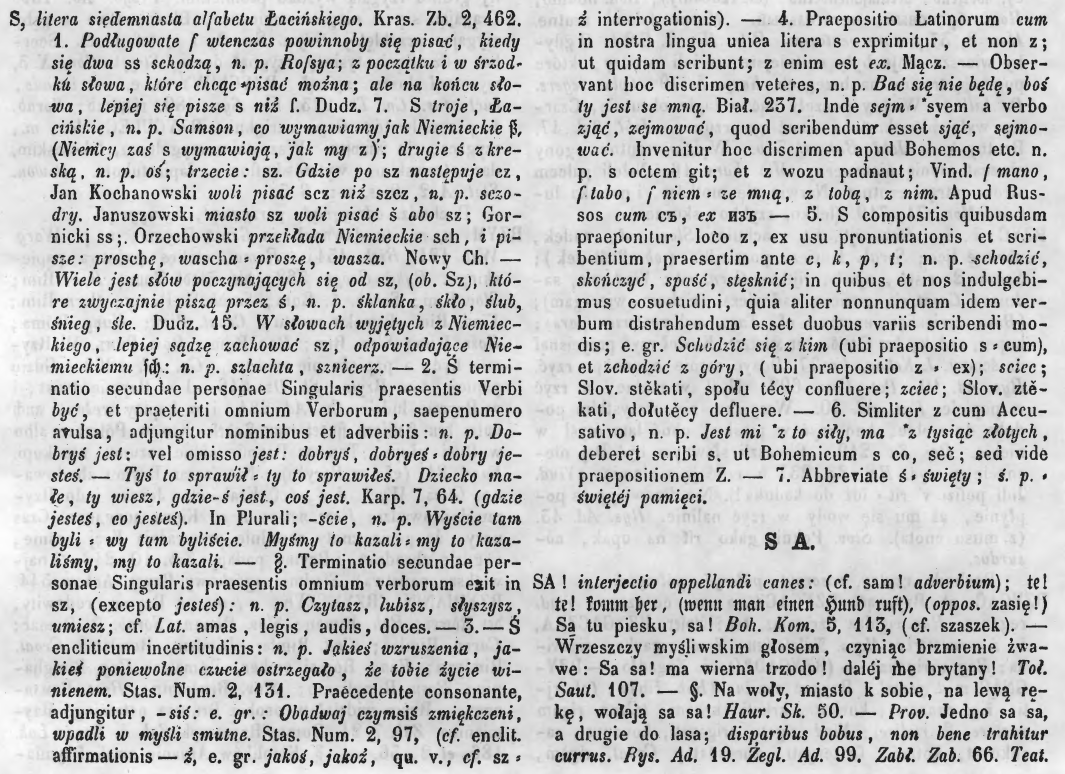
\includegraphics[scale=0.6]{linde-S.png}

\smallskip


\nin{}S, \textit{litera siedemnasta alfabetu Łacińskiego}. \biblio{Kras. Zb.}{Ignacy Krasicki}{Zbior potrzebnieyszych wiadomości porządkiem alfabetu ułożonych.}{2, 462}.\begin{description}
\item[1.] \textit{Podługowate ſ wtenczas powinnoby się pisać, kiedy
się dwa} ss \textit{schodzą}, \skrot{\textit{n. p.}}{n.p. = na przykład}{} \textit{Roſsya}; \nl\textit{z początku i w środku słowa, które chcąc pisać można}; \textit{ale na końcu słowa, lepiej się pisze} s \textit{niż}~ſ. \biblio{Dudz.}{Dudziński}{Zbiór rzeczy potrzebniejszych do wydoskonalenia języka.}{7}. \nl{}S \textit{troje, Łacińskie,} \skrot{\textit{n. p.}}{n.p. = na przykład}{} \textit{Samson, co wymawiamy jak Niemieckie} \niem{\textfrak{\ss}},
(\textit{Niemcy zaś} s \textit{wymawiają, jak my} z); \nl\textit{drugie} ś \textit{z kreską,} \skrot{\textit{n. p.}}{n.p. = na przykład}{} \textit{oś}; \nl\textit{trzecie}: sz. \nl\textit{Gdzie po} sz \textit{następuje} cz,
Jan Kochanowski \textit{woli pisać} scz \textit{niż} szcz, \skrot{\textit{n. p.}}{n.p. = na przykład}{}\textit{sczodry}. Januszowski \textit{miasto} sz \textit{woli pisać} š \textit{abo} sz; Gornicki ss; Orzechowski \textit{przekłada Niemieckie} \niem{sch}, {i pisze: pro}sch\textit{ę, wa}sch\textit{a} ⸗ \textit{proszę, wasza}. \biblio{Nowy Char.}{Jan Januszowski}{Nowy Charakter Polski}{}\nl —
\nl\textit{Wiele jest słów poczynających się od} sz, (\textit{ob}. Sz), \textit{które zwyczajnie piszą przez} ś, \nl\skrot{\textit{n. p.}}{n.p. = na przykład}{} \textit{śklanka, śkło, ślub, śnieg, śle}. \biblio{Dudz.}{Dudziński}{Zbiór rzeczy potrzebniejszych do wydoskonalenia języka.}{15}. \nl\textit{W słowach wyjętych z Niemieckiego, lepiej sądzę zachować} sz, \textit{odpowiadające Niemieckiemu} \niem{\textfrak{sch}}: \skrot{\textit{n. p.}}{n.p. = na przykład}{} \textit{szlachta, sznicerz}. \nl{}— 
\item[2.] Ś \lat{terminatio secundae personae Singularis praesentis Verbi}
\textit{być}, \lat{et praeteriti omnium Verborum, saepenumero avulsa, adjungitur nominibus et adverbiis}: \skrot{\textit{n. p.}}{n.p. = na przykład}{} \textit{Dobryś jest}: \lat{vel omisso} \textit{jest: dobryś, dobryeś} ⸗ \textit{dobry jesteś}.\nl — \nl\textit{Tyś to sprawił} ⸗ \textit{ty to sprawiłeś. \nl{}Dziecko małe, ty wiesz, gdzie-ś jest, coś jest.} \biblio{Karp.}{Franciszek Karpiński}{Zabawki wierszem i prozą}{7, 64}. (\textit{gdzie jesteś, co jesteś}). \nl\lat{In Plurali}; \textit{-ście,} \skrot{\textit{n. p.}}{n.p. = na przykład}{} \textit{Wyście tam byli} ⸗ \textit{wy tam byliście. Myśmy to kazali} ⸗ \textit{my to kazaliśmy, my to kazali}.\nl — \nl\reflectbox{§}. \lat{Terminatio secundae personae Singularis praesentis omnium verborum exit in}
sz, (\lat{excepto} \textit{jesteś}) \nl\skrot{\textit{n. p.:}}{n.p. = na przykład}{}\textit{Czytasz, lubisz, słyszysz, umiesz}; \nl{}\skrot{\lat{cf.}}{cf. (confer) = porównaj}{} \lat{\textit{Lat}. amas, legis, audis, doces}.\nl — \item[3.] — Ś
\lat{encliticum incertitudinis}: \nl\skrot{\textit{n. p.}}{n.p. = na przykład}{} \textit{Jakieś wzruszenia, jakieś poniewolne czucie ostrzegało, że tobie życie winienem}. \biblio{Stas. Num. 2}{Stasic}{Pochwała Marka Aureliusza}{131}. \nl\lat{Praecedente consonante,
adjungitur}, \textit{-siś: \nl\skrot{\lat{e. gr.}}{e.gr. (exempli gratia) = na przykład}{}: Obadwaj czymsiś zmiękczeni,
wpadli w myśli smutne}. \biblio{Stas. Num. 2}{Stasic}{Pochwała Marka Aureliusza}{97}, (\skrot{\lat{cf.}}{cf. (confer) = porównaj}{}\lat{enclit. affirmationis} — \textit{ż}, \skrot{\lat{e. gr.}}{e.gr. (exempli gratia) = na przykład}{} \textit{jakoś, jakoż}, \skrot{\lat{qu. v.}}{qu.v. (quod vide) = patrz też}{}, \skrot{\lat{\textit{cf.}}}{cf. (confer) = porównaj}{} sz ⸗ %e. gr. = exempli gratia 'na przykład'; qu. v. = quod vide 'patrz też'(dotyczy bieżącego dokumentu)
\textit{ż} \lat{interrogationis}).\nl — \item[4.] \lat{Praepositio Latinorum \textit{cum} in nostra lingua unica litera} s \lat{exprimitur, et non} z;
\lat{ut quidam scribunt}; z \lat{enim est \textit{ex}.} \biblio{Mącz.}{Jan Mączyński}{Lexicon Latino-Polonicum}{}\nl — \nl\lat{Observant hoc discrimen veteres}, \skrot{\textit{n. p.}}{n.p. = na przykład}{} \textit{Bać się nie będę, boś ty jest se mną}. \biblio{Biał.}{Białobrzeski}{X. Marc. Białobrzeskiego, bisk. Kamien. katechizm.}{237}. \nl\lat{Inde} \textit{sejm} ⸗ \textasteriskcentered{}syem \lat{a verbo}
\textit{zjąć, zejmować}, \lat{quod scribendum esset} \textit{sjąć, sejmować}. \nl\lat{Invenitur hoc discrimen apud Bohemos} \skrot{\lat{etc.}}{etc. (et cetera) = i tak dalej}{} \skrot{\textit{n. p.}}{n.p. = na przykład}{}% etc. = et cetera 'i tak dalej'
s octem git; \lat{et} z wozu padnaut; Vind. \textit{ſ mano}, % git - Nigella sativa? - Czarnuszka siewna? -> czarnuszka z octem? (czyżby środek leczniczy?)
\textit{ſ tabo, ſ niem} ⸗ \textit{ze mną, z tobą, z nim}. \nl\lat{Apud Russos \textit{cum}} \rus{cъ}, \lat{\textit{ex}} \rus{изъ}\nl — \item[5.] S \lat{compositis quibusdam praeponitur, loco} z, \lat{ex usu pronuntiationis et scribentium, praesertim ante} \textit{c, k, p, t}; \nl\skrot{\textit{n. p.}}{n.p. = na przykład}{} \textit \textit{schodzić},
\textit{skończyć}, \textit{spaść}, \textit{stęsknić}; \nl\lat{in quibus et nos indulgebimus cosuetudini, quia aliter nonnunquam idem verbum distrahendum esset duobus variis scribendi modis;} \skrot{\lat{e. gr.}}{e.gr. (exempli gratia) = na przykład}{} \textit{Schodzić się z kim} (\lat{ubi praepositio} s ⸗ \lat{cum}),
\lat{et} \textit{zchodzić z góry}, (\lat{ubi praepositio} z ⸗ \lat{ex});\nl \textit{sciec};
Slov. \slov{stěkati, społu técy} \lat{confluere}; \nl\textit{zciec}; Slov. \slov{ztěkati, dołutěcy} \lat{defluere}.\nl — \item[6.] \lat{Simliter z cum Accusativo}, \skrot{\textit{n. p.}}{n.p. = na przykład}{}\textit{Jest mi \textasteriskcentered{}z to siły, ma \textasteriskcentered{}z tysiąc złotych},
\lat{deberet scribi} s. \nl\lat{ut Bohemicum} s co, seč; \lat{sed vide
praepositionem} Z.\nl — \item[7.] \lat{Abbreviate} ś ⸗ \textit{święty}; \textit{ś. p.} ⸗ \textit{świętéj pamięci}.
\end{description}





\end{document}

%%% Local Variables: 
%%% coding: utf-8-unix
%%% mode: latex
%%% TeX-master: t
%%% TeX-PDF-mode: t
%%% TeX-engine: xetex
%%% End: 
